% Adapted from the instructor-provided Fall 2026 report template.
\documentclass[12pt,letterpaper]{report}
\usepackage[T1]{fontenc}
\usepackage{amsmath,amssymb,amsfonts}
\usepackage{graphicx,booktabs,listings,xcolor,longtable,array}
\usepackage[margin=1in]{geometry}
\usepackage{setspace}
\usepackage[hidelinks]{hyperref}
\renewcommand{\bibname}{References}
\onehalfspacing
\setlength{\emergencystretch}{3em}
\lstset{basicstyle=\ttfamily\footnotesize,breaklines=true,columns=fullflexible,
  keepspaces=true,showstringspaces=false,frame=none,aboveskip=10pt,belowskip=10pt}
\graphicspath{{assets/}}
\newcommand{\file}[1]{\path{#1}}
\newcommand{\workinghash}{\texttt{D54886033D5ED8E6B9BA5C58EF60A414}\\\texttt{C3F2202BD1A2F6A5A7D407D499BCA5C7}}
\begin{document}
\hypersetup{pageanchor=false}
\begin{titlepage}
\centering
{\LARGE Fayetteville State University}\\[0.5em]
{\large Department of Mathematics and Computer Science}\\[2.5em]
{\LARGE\bfseries NTFS Filesystem Steganography and Forensic MFT Parser}\\[1.5em]
{\large CS481 Capstone Project --- Final Report}\\[0.5em]
{\large Fall 2026}\\[2em]
\textbf{Team 3}\\[1em]
\begin{tabular}{@{}lll@{}}
\toprule Role & Name & Student ID\\\midrule
Team Leader & Lucas Curtis & 830849238\\[1em]
Team Member & Jeff Perez & 830822886\\\bottomrule
\end{tabular}\\[2em]
\textbf{Supervisor:} Professor Xianping Wang\\[0.7em]
\textbf{Date of Submission:} November 29, 2026
\vfill
\url{https://github.com/Lcurtis1Broncos/CSC-481-Capstone-Group}\\
Code release: \file{v1.0-final}
\end{titlepage}
\pagenumbering{roman}
\hypersetup{pageanchor=true}
\chapter*{Declaration of Originality}
\addcontentsline{toc}{chapter}{Declaration of Originality}
We declare that the submitted report and accompanying project accurately
represent our work and contributions. External sources, technical definitions,
and ideas are acknowledged using numeric citations. We have reviewed the
reported experiments, limitations, and contribution records. We distinguish
new experiments from historical evidence and do not claim unperformed tests.
AI assistance was used for drafting, code support, and formatting. The
authors are responsible for checking the sources, software, and claims and
for ensuring this assistance complies with university and course policy
before signing.

\vspace{2em}
\noindent Lucas Curtis\\[1em]
Signature: \rule{2.8in}{0.4pt}\quad Date: \rule{1in}{0.4pt}\\[2em]
Jeff Perez\\[1em]
Signature: \rule{2.8in}{0.4pt}\quad Date: \rule{1in}{0.4pt}

\chapter*{Abstract}
\addcontentsline{toc}{chapter}{Abstract}
Information concealed in NTFS alternate data streams and file slack can be
missed by examinations limited to ordinary filenames and logical file
contents. This project investigates whether a small read-only Python tool
can expose the relevant filesystem structures and recover controlled hidden
payloads while preserving its source image. The implementation parses
partition and boot metadata, selected Master File Table attributes, resident
streams, nonresident data runs, and bounded final-cluster slack. It exports
payloads to separate files and records expected and actual lengths, SHA-256
hashes, and image-integrity results. A dedicated Windows VirtualBox laboratory
provided eight baseline files, a 36-byte named-stream marker, and a 25-byte
slack marker. Historical validation matched all eight file lengths and both
hidden-payload hashes. On November 25, the team confirmed original/recovered
SHA-256 matches for all eight baseline files. Release verification passed 68 automated tests and seven
end-to-end acceptance checks. An additional campaign recovered 50 synthetic
slack payloads exactly, agreed with a direct-byte-read baseline in all 50
cases, and detected all 50 deliberately introduced single-bit payload changes
as integrity failures. A separate 100-image detection experiment measured
100\% ADS detection with 40\% false positives; slack signature search measured
60\% detection and 40\% evasion with no false positives. These fixed-rule
results describe constructed known-record cases, not general steganalysis
or universal NTFS support. The expanded suite passed 73 tests. Fragmented
MFT storage and several advanced attribute types remain
unsupported. The project provides a reproducible educational workflow whose
claims are bounded by recorded evidence and explicit limitations.

\vspace{1em}
\noindent\textbf{Keywords:} NTFS; alternate data streams; file slack;
Master File Table; forensic recovery; evidence integrity.
\tableofcontents
\listoffigures
\listoftables
\clearpage
\pagenumbering{arabic}
\chapter{Introduction}
\section{Background}
Digital forensic examination depends on understanding what a storage format
makes visible and what a particular tool chooses to display. A normal file
listing is useful for navigation, but it is not a complete representation of
the bytes associated with an NTFS file. Microsoft documents files as having
one default stream and potentially additional named streams \cite{streams,clusters}.
For this project, the distinction matters because an examiner who exports
only the default stream can recover a valid-looking host file while omitting
the controlled information attached to it.

Information hiding also has a longer history than digital filesystems.
Anderson describes historical concealed messages and distinguishes passive
observers from opponents able to modify communications \cite{anderson}.
The relevant lesson for this laboratory is methodological: successfully
storing a hidden message does not establish that it will remain secret,
survive alteration, or be recoverable under every acquisition method. Each
claim requires its own experiment. Our work addresses recovery and integrity
in a deliberately limited storage environment.

The second location examined here is final-cluster file slack: bytes after
logical content ends in its final allocated cluster. We established a known
marker's presence through recovery and comparison with its earlier recorded
hash, rather than inferring it solely from unused capacity.

\section{Problem Statement}
The project asks whether a purpose-built Python parser can interpret the
necessary structures in a controlled raw NTFS image, locate documented ADS
and slack payloads, and recover them without changing the source image.
A related problem is how to report the strength of the evidence: successful
file identification, matching length, matching original hash, and unchanged
source image support different conclusions and must not be merged into one
unqualified success claim.

The contribution is an inspectable educational workflow connecting on-disk
offsets, extraction decisions, and verification reports. It does not claim
that mature tools lack ADS or slack capabilities.

\section{Aims and Objectives}
The overall aim is to demonstrate controlled NTFS information hiding and
defensive recovery with evidence that another reader can inspect. Six
measurable objectives guide the evaluation:
\begin{enumerate}
\item To characterize the laboratory image by recording its hash, partition
start, sector and cluster sizes, MFT location, and record size.
\item To identify the eight known baseline files and compare their names and
logical lengths with independently recorded Windows values.
\item To document a named ADS marker and a bounded slack marker, including
their lengths, locations, and expected SHA-256 values.
\item To recover both hidden markers exactly while retaining the original
source image and writing outputs to separate new files.
\item To test malformed inputs, unsupported layouts, output protection, and
verification outcomes using reproducible automated cases.
\item To package the source, dataset-generation scripts, instructions, and
results so a fresh checkout can reproduce the supported workflow.
\end{enumerate}

Original/recovered SHA-256 matches for all eight ordinary files were
confirmed by the team on November 25. These comparisons remain separate
from the independently documented hidden-marker comparisons.

\section{Project Scope and Limitations}
The primary experiment uses a dedicated VirtualBox NTFS disk exported as a
raw image. The implementation supports selected in-use MFT records,
resident data, ordinary nonresident extents, exact named-stream selection,
and bounded reads from the final cluster's slack. It does not reconstruct
deleted files, decrypt BitLocker or EFS, resolve attribute lists, or traverse
arbitrary fragmented MFT storage. A successful controlled experiment is not
evidence of compatibility with every NTFS volume.

Handcrafted NTFS-shaped fixtures exercise supported paths without the
large image; they are not mountable Windows filesystems. The 50 synthetic
payload samples vary bytes and lengths within one layout, rather than
representing independently acquired volumes.

Two fixed detection rules were evaluated separately on 100 labeled synthetic
images: named-stream screening and a known-marker search in calculated slack.
Their measured false-positive and evasion rates apply only to the constructed
cases and selected records. No statistical steganalysis classifier,
confidentiality layer, or general unknown-payload detector was implemented.
Chapter 5 explains the measured storage and detection metrics and why a
visual-quality score is not applicable to this filesystem carrier.

\section{Thesis Outline}
Chapter 2 reviews information hiding, NTFS structures, and relevant tools.
Chapter 3 defines the architecture, extraction rules, formulas, and
experimental design. Chapter 4 explains the code and development challenges.
Chapter 5 presents historical laboratory results and the new synthetic
campaign. Chapter 6 examines attacks and limitations. Chapter 7 evaluates
the objectives and proposes future work. The appendices provide execution
instructions, raw results, and the development record.

\section{Responsible Disclosure and Ethical Use Statement}
The software and experiments are intended solely for education, research,
and defensive analysis of authorized data. All hiding operations were
restricted to dedicated laboratory material or newly generated fixtures.
The tools must not be used for malicious concealment, unauthorized access,
or alteration of another person's evidence. Recovery should operate on
preserved images, with separate destinations for generated files.

NIST places forensic activity within an organization's documented process
\cite{nist86}. Accordingly, image identities and evidence gaps are retained.
This project is not certified for operational casework. No third-party
vulnerability requiring disclosure was discovered.

\chapter{Literature Review and Related Work}
\section{History of Steganography}
Classical examples of steganography rely on concealing the existence of a
message inside an apparently ordinary object or communication. Anderson's
account includes messages hidden beneath writing surfaces and distinguishes
concealment from making content unreadable \cite{anderson}. The present
project uses the same broad question at a filesystem boundary: which bytes
are omitted by a routine view of a file? It does not implement the
cryptographic constructions discussed in that work.

The transition to digital media created several possible carriers, including
images, audio, documents, and system storage. Petitcolas's information-hiding
resource distinguishes applications such as watermarking, fingerprinting,
covert channels, and hidden-information detection \cite{petitcolas}.
Those applications have different objectives. A watermark may be intended
to survive ordinary processing, whereas a forensic training marker is useful
when it provides a known expected answer. Our plaintext markers were selected
for traceability, not for strong concealment against an informed examiner.

Filesystem hiding is also different from image-bit substitution. It relies
on how storage structures expose or omit byte ranges, rather than on a
perceptual model of pixels. This difference drives the evaluation: capacity
can be expressed in bytes, while correctness requires reconstructing the
appropriate stream or slack range. A perceptually unchanged document is not
by itself evidence that all associated storage bytes are unchanged.

\section{NTFS Structures Relevant to Recovery}
Microsoft describes the Master File Table as the structure holding
information needed to retrieve files. File records contain typed attributes,
and a file can require more than one record \cite{mft}. This supports a
metadata-driven approach: recovery begins by identifying an appropriate
record and attribute rather than searching blindly for a familiar content
signature. It also establishes a boundary for the project, because resolving
additional attribute records was not implemented.

The file-record header identifies the first attribute, flags, and the
relationship to a base record \cite{record}. The implementation checks those
fields before exporting content. Attribute headers distinguish resident
values from nonresident values and identify named attributes \cite{attribute}.
Our design treats this distinction as a branching point. Resident bytes
come from the validated record; nonresident bytes require mapping pairs.
Confusing the branches would produce an incorrect offset or an incomplete
recovery.

The update sequence array protects multisector structures by replacing and
later restoring sector-tail words. Microsoft's description requires checking
the sequence values before restoring saved words \cite{usa}. This is
especially important for resident content crossing a sector boundary.
Reading its apparent raw range without restoration can include the transfer
sequence word instead of the original content. The recovery implementation
therefore uses fixup-restored records, and the automated suite includes
a resident-content case crossing that boundary.

The standard-information attribute and filename attribute supply different
metadata roles \cite{standard,filename}. The project reports timestamps,
flags, and names for context, but selects actual content through
\file{$DATA}. During validation, filename metadata sizes did not always
agree with current data-stream sizes. We retained this distinction in the
reporting rules instead of treating every size field as interchangeable.

\section{Streams and Allocation Semantics}
Each NTFS stream has its own allocation, actual size, and valid-data length
\cite{streams}. Those concepts matter both for recovering ordinary content
and for avoiding disclosure of bytes the filesystem would not present as
initialized content. Microsoft documents that reads between valid-data
length and logical end return zeros \cite{fsutilfile}. Our recovery path
follows that semantic distinction: initialized bytes are read from mapped
extents, then any required logical tail is generated as zeros.

Final-cluster slack is a separate selection. Its start follows the logical
end in the last cluster that contains content. Recovering a normal file
should stop at its logical size; recovering a known slack marker should
explicitly request a bounded range outside that content. This separation
prevents a file export from silently mixing document bytes with hidden or
residual material.

\section{Related Systems and Tools}
\subsection{Sysinternals Streams}
Streams enumerates named streams associated with live files and directories;
its official documentation provides the stream-name syntax and command
options \cite{sysstreams}. It offers a straightforward way to expose ADS
on a mounted NTFS volume. The project differs in working from a raw image
and showing how the named attribute leads to the recovered bytes. Streams
was reviewed as related work, not benchmarked in this campaign.

\subsection{The Sleuth Kit}
The Sleuth Kit provides image-oriented filesystem analysis, including NTFS
attributes and alternate streams \cite{tsk}. Its \file{icat} utility can
export content by metadata address and optionally include slack
\cite{icat}. These capabilities directly overlap the broad recovery task.
Our implementation does not claim a new category of extraction capability.
Its smaller scope permits close inspection of a selected record, the
derived extents, the expected payload, and the resulting JSON report.

\subsection{Autopsy}
Autopsy provides a broader analysis environment around filesystem
capabilities, including case management and automated operations
\cite{tsk}. Such integration is valuable in a full investigation, where
organizing evidence and correlating findings matter alongside extraction.
Our command-line workflow does not replace that environment. The project
instead exposes a narrow teaching sequence that can be demonstrated without
introducing a complete case-management system.

\subsection{PhotoRec}
PhotoRec uses underlying data and recognized file formats rather than
depending entirely on filesystem metadata \cite{photorec}. This can help
when metadata is damaged, but it answers a different starting question
from selecting a named attribute in an intact record. For the deliberately
small plaintext markers in this experiment, a documented stream identity
and length provide a more direct oracle than a file-format signature.
No measured superiority over PhotoRec is asserted.

\section{Forensic Validation and Evidence Strength}
NIST's Computer Forensics Tool Testing program emphasizes specifications,
procedures, criteria, and test sets for examining tool reliability
\cite{cftt}. The project adopts that general testing discipline at a student
scale: supported outcomes are written down, failure conditions are exercised,
and test inputs are reproducible. It has not undergone CFTT certification
or an independent validation program.

SHA-256 is used as an integrity check, following the digest concept defined
by the Secure Hash Standard \cite{sha}. A recovered file's digest has its
strongest practical role when compared with a separately recorded expected
digest. Hashing an output after extraction establishes an identifier for that
output, but does not retrospectively establish its agreement with an unknown
original. For this reason, the earlier baseline-file content comparisons remained
unverified until the team confirmed the original hash matches on November 25.

\section{Gap Analysis and Project Rationale}
The reviewed tools already address ADS enumeration, raw-image examination,
or content recovery. The gap addressed here is instructional transparency
and reproducibility within the semester project. The implementation joins
raw geometry, record validation, named-stream selection, bounded slack
extraction, and explicit expected-value reporting in one inspectable path.
It avoids dependence on a mounted original disk for recovery.

That choice trades breadth for a clearer explanation of supported behavior.
It also creates identifiable weaknesses: a known-record workflow does not
find every hidden payload, and a handcrafted fixture does not reproduce
Windows allocation behavior. Those weaknesses are not shortcomings proved
against the reviewed mature tools. They are limitations of this project's
scope and evidence. The comparison in Chapter 5 therefore uses a simple,
actually executed direct-byte-read baseline, while the tools reviewed here
remain qualitative context.

\chapter{System Design and Methodology}
\section{High Level Architecture}
The architecture separates laboratory preparation from evidence recovery.
Preparation creates identifiable image states and records original marker
values. Recovery opens the selected image for reading, validates the required
structures, and writes recovered bytes and a report elsewhere. Figure
\ref{fig:architecture} shows this separation. The image passed to the reader
is an artifact of preparation; recovery never calls the embedding routine.

\begin{figure}[htbp]
\centering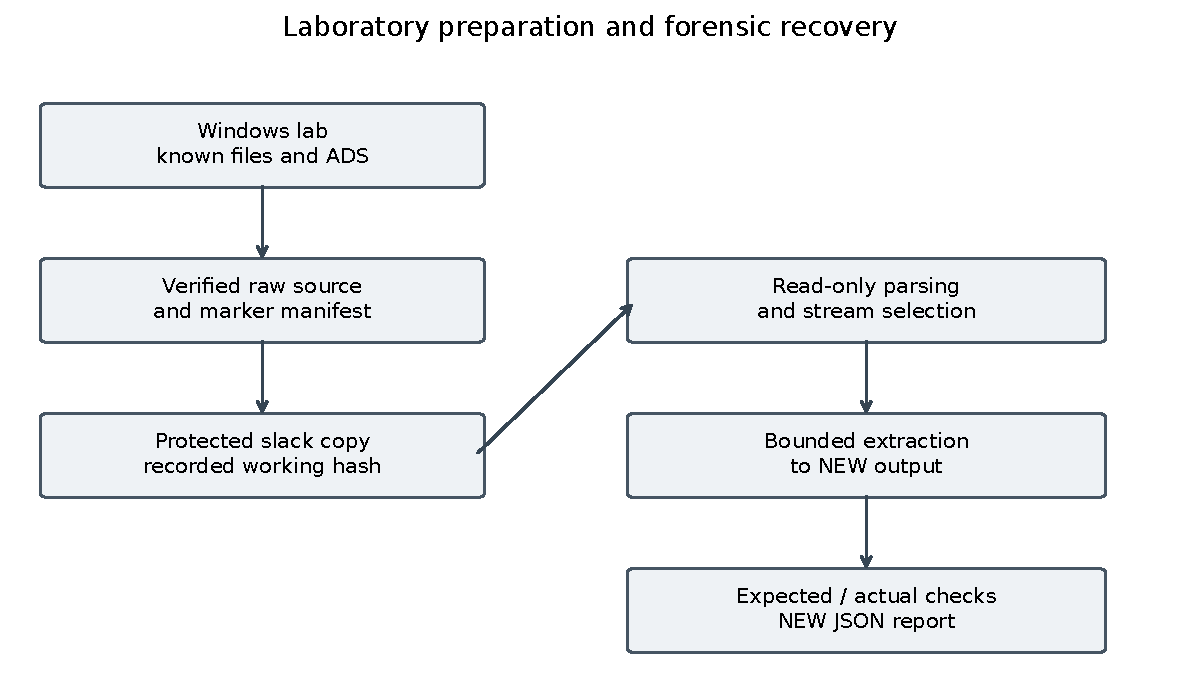
\includegraphics[width=\textwidth]{architecture.pdf}
\caption{Preparation and recovery data flow with separate output files.}
\label{fig:architecture}
\end{figure}

ADS creation took place inside the Windows guest. Slack embedding changed
only a documented range in a protected image copy. The manifest linked image
hashes, host record, payload length, offset, and original payload hash before
the later recovery comparison.

The portable fixture constructs metadata and original bytes directly so
tests can run without the large laboratory disk. Its generated expectations
remain distinct from independently recorded Windows evidence.

\section{Addressing Model and Mathematical Definitions}
Let $P$ be the NTFS partition's absolute byte offset, $B$ the bytes per sector,
$S$ the sectors per cluster, $C$ the cluster size, $L$ a logical cluster
number, and $R$ the MFT record size. The implementation uses:
\begin{align}
C &= B S,\\
O_{\mathrm{cluster}} &= P + LC,\\
O_{\mathrm{MFT}} &= P + L_{\mathrm{MFT}} C,\\
O_{\mathrm{record}}(n) &= O_{\mathrm{MFT}} + nR.
\end{align}
The last equation assumes supported contiguous MFT storage. Recovery checks
that assumption instead of treating it as valid for arbitrary images.
The metadata reader's simpler selected-record path has a narrower validation
guarantee, as discussed in Chapter 6.

For the Windows laboratory, $P=1{,}048{,}576$, $C=4{,}096$, and
$L_{\mathrm{MFT}}=786{,}432$, giving
$O_{\mathrm{MFT}}=3{,}222{,}274{,}048$. These are measured properties of the
controlled image, not universal NTFS constants. The generated fixture instead
uses 512-byte clusters and a much smaller MFT location.

For a nonempty ordinary stream of logical size $F$, final-cluster slack has
length
\begin{equation}
Q = (C - (F \bmod C)) \bmod C.
\end{equation}
If $Q=0$, there is no final-cluster tail to select. For a fragmented file,
the final logical cluster must be resolved through the run sequence. Adding
$F$ to the first physical extent is valid only when that extent actually
contains the relevant logical position. The tests include a negative LCN
delta so this distinction is exercised rather than assumed.

If $A$ is the absolute start of the final physical cluster containing
logical content, slack begins at $A+(F\bmod C)$ when the remainder is nonzero.
For the laboratory document, $F=13{,}437$ and $C=4{,}096$, so the remainder
is 1,149 and $Q=2{,}947$. The selected marker starts at byte 16,049,277.
A request with relative slack offset $d$ and length $N$ must satisfy
$d\geq0$, $N>0$, and $d+N\leq Q$.

Capacity is reported in bytes and bits for this storage carrier. Occupancy
is $100N/Q$ percent of the available final-cluster tail, not bits per pixel.
For the 25-byte laboratory marker this is approximately 0.8483\% of the
2,947-byte tail. That percentage is measured use of this location, not a
maximum ADS capacity or a filesystem-wide concealment rate.

\section{Embedding Algorithm}
The manual ADS procedure writes the known marker to the named stream
\file{hostfile.txt:CapstoneEvidence}, measures its exact length, and records
its hash. The host path and stream name are part of the experiment's identity.
No assumption is made that reading the unnamed host stream retrieves the ADS.

The controlled slack-copy algorithm is summarized below. It is deliberately
more restrictive than a general disk editor: the source must match the known
laboratory image, the chosen record must represent a supported file, and
the destination must be new.
\begin{lstlisting}
require source hash equals documented lab hash
require destination is new and distinct from source
read partition, boot geometry, record, and restored attributes
require one supported unnamed nonresident data stream
decode runs and calculate final logical cluster and slack
require marker fits entirely inside that final-cluster tail
copy source to destination; change only selected marker bytes
compare complete copy with source plus intended marker range
save source hash, copy hash, marker hash, and location manifest
\end{lstlisting}
The complete comparison supports a specific preservation claim: all bytes
outside the designated range match the source. It does not claim that the
working image itself is unchanged, because embedding intentionally changes it.
Recovery integrity is evaluated later, relative to that working image.

\section{Extraction and Verification Algorithms}
Extraction first selects the content's identity and then copies its bytes.
The identity is a record number and exact stream name, with an optional
slack-relative selection. This prevents an empty or default stream name from
silently standing in for the requested ADS.
\noindent\begin{minipage}{\linewidth}
\begin{lstlisting}
validate image geometry and supported MFT coverage
read selected record; validate flags and sector-tail fixups
parse attributes; reject unsupported extensions or stream flags
select exactly one DATA stream with requested name
if resident: use value from restored record
otherwise: decode runs in logical order and validate bounds
if slack requested: resolve final cluster and bound selected range
require source, output, and report paths are distinct
require output and report do not already exist
hash source before extraction; export to new output
compare output length/hash with independently supplied expectations
hash source after extraction; save result and errors
\end{lstlisting}
\end{minipage}

For ordinary nonresident streams, export is limited to initialized content
followed by zero bytes up to logical end where required. It does not append
slack. A slack request is an explicit alternate selection with its own length
and a report field preserving the host's logical size. This allows the
reviewer to distinguish a 25-byte recovered marker from a 13,437-byte host.

Verification has three separate comparisons. The expected-image comparison
identifies the selected source when an expected image hash is supplied.
The before/after comparison checks observed source preservation during the
run. The recovered-payload comparison checks expected content and size.
These comparisons address different failure modes; none should be described
simply as an undifferentiated hash match.

\section{Report Schema and Selection Metadata}
No custom network protocol or embedded packet header is used. The markers
are plain byte strings, and the metadata needed to find them is supplied
through manifests and CLI parameters. Table \ref{tab:schema} describes the
report fields that play the relevant coordination role. Their lengths are
not represented as fixed binary header sizes because the report is JSON.

\begin{table}[htbp]\centering\small
\caption{Verification report fields and their interpretation.}\label{tab:schema}
\begin{tabular}{p{2.15in}p{3.8in}}\toprule
Field & Interpretation\\\midrule
\file{record_number}, \file{stream_name} & Selected metadata identity.\\
\file{recovery_kind} & Ordinary stream or bounded slack payload.\\
\file{extents} & Absolute byte ranges used for a nonresident export.\\
\file{host_logical_size} & Host size retained for a slack selection.\\
\file{expected_length}, \file{expected_sha256} & Independent payload expectations.\\
\file{recovered_length}, \file{recovered_sha256} & Measured output values.\\
\file{source_image_hash_match} & Agreement with supplied expected image hash.\\
\file{source_unchanged} & Agreement of source hashes before and after export.\\
\file{overall_result}, \file{errors} & Decision and diagnostic information.\\\bottomrule
\end{tabular}\end{table}

\section{Security Model}
The examiner is assumed to possess an authorized stable image and a trusted
expectation manifest. An adversary may know the hiding method, observe the
plaintext markers, or alter accessible storage bytes. No secret key prevents
them from reading a known marker. The trust boundary is therefore around
evidence preservation and the provenance of expectations, not cryptographic
confidentiality.

Malformed metadata should be refused. Before/after hashing neither locks
the source nor proves its creator; stable preserved storage remains an
operational assumption.

\section{Experimental Design}
Three evidence layers are used. Historical Windows checks establish image
geometry, eight file lengths, and the two marker recoveries. Automated tests
exercise valid and invalid structures in small inputs. The final report
campaign constructs 50 slack payloads: ten deterministic samples at each
of 1, 25, 100, 200, and 324 bytes in a 324-byte synthetic slack region.
The random seed is fixed at 4,812,026 so the bytes can be regenerated.

Each sample is first recovered unchanged and compared byte-for-byte with
its separately written original. The baseline independently reads the known
construction offset without parsing metadata. A second new image changes
one bit in the first payload byte; recovery uses the changed image's correct
hash but retains the original payload expectation. This isolates payload
integrity failure from wrong-image identification. It is not an experiment
in attack-resistant concealment.

Bit error rate is defined as
\begin{equation}
\mathrm{BER}=100\frac{\sum_{i=1}^{N}\operatorname{popcount}(x_i\oplus y_i)}{8N}\%.
\end{equation}
Clean exact matches should have BER zero. One changed bit should yield
$100/(8N)$ percent and a failed payload comparison. Timing values are
recorded for single in-process runs on tiny cached inputs, with reporting
and hashing included for the structured path. They are not storage-throughput
benchmarks.

\subsection{Detection and Evasion Experiment}
A separate November 25 experiment applies two fixed screening rules to
100 newly constructed images, using seed 4,811,125. The ADS rule flags any
named data stream in the selected record. The slack rule searches the
entire calculated final-cluster tail for the known 25-byte marker; it does
not receive the planted offset. Neither rule receives the construction
label or an expected payload hash. This evaluates discovery rules rather
than reusing recovery-integrity decisions as detection results.

The ADS group contains 25 intentionally hidden named streams, ten legitimate
named-stream controls, and 15 ordinary-file controls. The slack group contains
15 plaintext markers, ten reversibly XOR-transformed markers, 15 random-tail
controls, and ten controls containing the marker only in logical file data.
The XOR transformation changes each marker byte with constant \file{0x5A};
it is a simple signature challenge, not encryption or a claim of strong secrecy.
Labels are assigned by construction before either detector runs. All images
share one synthetic layout; they are not independent Windows-formatted volumes.

For intentionally hidden content as the positive class, define true positives
($TP$), false negatives ($FN$), false positives ($FP$), and true negatives
($TN$). A legitimate named stream flagged for review is an $FP$ relative to
this hidden-content label, even though its stream enumeration is correct.
The following percentages use separate denominators for each rule:
\begin{align}
\mathrm{Accuracy} &= 100\frac{TP+TN}{TP+TN+FP+FN},\\
\mathrm{Detection} &= 100\frac{TP}{TP+FN},\\
\mathrm{FPR} &= 100\frac{FP}{FP+TN},\\
\mathrm{Evasion} &= 100\frac{FN}{TP+FN}.
\end{align}
Evasion means a hidden-positive case missed by that particular rule.
Malformed inputs abort the experiment rather than being counted as clean
negatives. Before/after SHA-256 checks verify that screening preserves each
source. The Windows image supplies two additional known-positive checks,
not a real-volume negative-rate estimate.

\chapter{Implementation Details}
\section{Development and Validation Environment}
The main laboratory consisted of a Windows guest in VirtualBox, a dedicated
approximately 8 GiB virtual disk, and exported raw images. The release and
final report campaign were validated on Windows 11, build 26300, with
Python 3.15.0. The current host reports an Intel Core i5-8365U processor at
1.60 GHz and 7.81 GiB of OS-reported physical memory. The historical guest's
exact Windows build, VirtualBox version, and RAM allocation were not retained
in the experiment evidence. Consequently no hardware-normalized performance
claim is made.

Production code uses Python's standard library, including \file{argparse},
\file{dataclasses}, \file{datetime}, \file{hashlib}, \file{json}, and
\file{pathlib}. The test suite uses \file{unittest}, \file{tempfile}, and
\file{subprocess}. There are no third-party runtime dependencies; these
modules therefore share the interpreter version rather than separate package
versions. Python 3.11 or later is the documented minimum. The final campaign
also uses standard-library CSV, random-number generation, and timing.

Git provides the version history and release identity. The verified code
package is commit \file{06eb0ff}, tagged \file{v1.0-final}. Report-specific
experiments were added subsequently on a separate report branch. This
distinction prevents the final campaign from being silently represented as
part of the earlier release's acceptance run.

\section{Code Architecture}
The code is organized as small procedural modules around a shared location
representation. \file{ntfs_image_reader.py} supplies geometry, metadata,
attribute, run, and slack calculations. \file{ntfs_recovery.py} adds stricter
recovery validation, stream selection, bounded export, and verification
reporting. \file{slack_embed.py} is the separate write-capable laboratory
preparation utility. Figure \ref{fig:callgraph} summarizes their relationships.

\begin{figure}[htbp]\centering
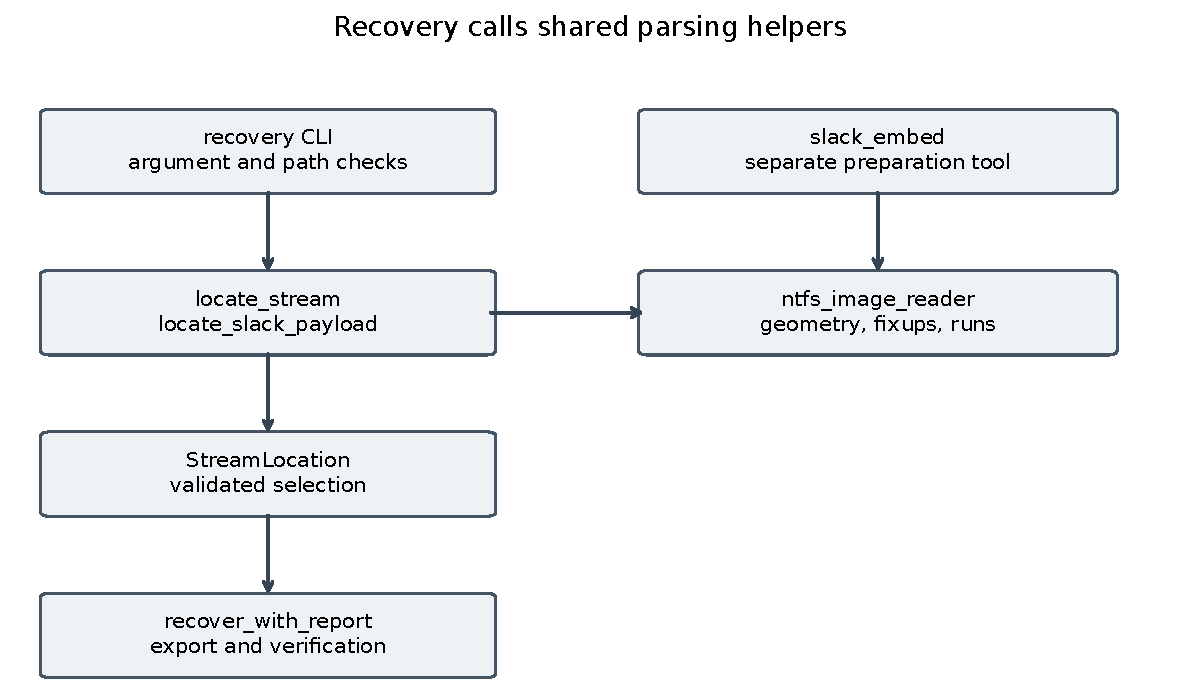
\includegraphics[width=\textwidth]{callgraph.pdf}
\caption{Module call relationships for recovery and laboratory preparation.}
\label{fig:callgraph}\end{figure}

\file{StreamLocation} is an immutable data class recording the source path,
record and filename, stream identity, logical and initialized sizes,
resident content or nonresident extents, and optional slack metadata.
An immutable location makes selection explicit before writing output.
It does not freeze the underlying source file, so source stability must still
be maintained and checked.

The report workflow separates preflight errors from errors encountered after
creating output artifacts. Invalid arguments, colliding destinations, or
an out-of-range selection are refused early. An error during export can
leave a diagnostic report or partial output. Such an artifact is not a
successful recovery and must not be relabeled as one merely because a file
exists. Reruns use new filenames rather than silently replacing evidence.

\section{Key Code Snippets}
\subsection{Restoring Record Sector Tails}
Listing \ref{lst:fixup} reproduces the central loop of the shared fixup
routine. Earlier checks validate record geometry, the update-sequence count,
and array bounds. For each protected sector, the observed tail must equal
the expected sequence word before the original word is restored. The routine
returns new bytes rather than editing the source image.

\begin{lstlisting}[language=Python,caption={Sector-tail validation and restoration from the release source.},label={lst:fixup}]
restored = bytearray(record)
sequence = record[usa_offset : usa_offset + 2]
for index in range(1, usa_count):
    tail = index * sector_size - 2
    if record[tail : tail + 2] != sequence:
        raise ValueError("MFT sector-tail fixup validation failed.")
    restored[tail : tail + 2] = record[
        usa_offset + index * 2 : usa_offset + index * 2 + 2]
return bytes(restored)
\end{lstlisting}

The important failure case is a mismatch, not just an invalid signature.
A record can begin with \file{FILE} yet still fail multisector validation.
Recovering resident data directly from such a record would ignore evidence
of an incomplete or inconsistent transfer. The project explicitly tests
restoration and refusal, following the documented role of the update
sequence array \cite{usa}.

\subsection{Bounding a Slack Selection}
Listing \ref{lst:slack} shows the decisive boundary check and conversion from
slack-relative position to an absolute byte offset. It follows validation of
the requested integer values and host stream. The returned location retains
the host size while selecting only the requested payload bytes.

\begin{lstlisting}[language=Python,caption={Slack selection bounds from the release recovery module.},label={lst:slack}]
host = locate_stream(image, record_number, stream_name)
if host.resident_value is not None or host.slack is None:
    raise ValueError("Selected stream has no supported final-cluster slack.")
if relative_offset + payload_length > host.slack["length"]:
    raise ValueError("Requested payload extends outside the calculated slack range.")
offset = host.slack["byte_offset"] + relative_offset
if offset + payload_length > host.image.stat().st_size:
    raise ValueError("Requested slack payload exceeds the image.")
\end{lstlisting}

This check prevents a caller from using slack mode as an arbitrary
unbounded disk read. It also demonstrates why the selected marker length
must be distinguished from the entire available tail. In the Windows lab,
25 bytes were requested from a 2,947-byte slack region. In the synthetic
campaign, the maximum valid selection was 324 bytes, and a 325-byte request
was refused in the acceptance workflow.

\subsection{Reading Nonresident Content}
Listing \ref{lst:extent} reproduces the core bounded read loop. Extents are
already ordered by logical position. Each read must return the requested
number of bytes; otherwise the source is treated as truncated. After the
initialized part is exhausted, the remaining logical tail is supplied as
zero bytes in the surrounding function.

\begin{lstlisting}[language=Python,caption={Bounded extent reads from the release recovery module.},label={lst:extent}]
for offset, length in location.extents:
    source.seek(offset)
    extent_remaining = min(length, remaining)
    while extent_remaining:
        size = min(CHUNK_SIZE, extent_remaining)
        chunk = source.read(size)
        if len(chunk) != size:
            raise ValueError("Source was truncated during recovery.")
        yield chunk
        remaining -= size
        extent_remaining -= size
    if not remaining:
        break
\end{lstlisting}

Neither physical adjacency nor increasing disk offsets are required for
ordinary file extents. A later logical run can be earlier on disk. The
negative-delta fixtures and fragmented-file test are therefore important
checks of ordering, independent of the specific lab file's simpler layout.

\section{Challenges and Solutions}
\subsection{Encrypted Initial Baseline}
The first image's target partition began with \file{-FVE-FS-}, not a directly
parseable NTFS boot identifier. Its hash could still be valid; hashing alone
did not make its content suitable for the planned parser. The solution was
to retain that attempt in the evidence log and recreate an unencrypted
baseline. The project did not implement BitLocker decryption or reinterpret
the encrypted bytes as ordinary NTFS structures.

\subsection{Rounded Sizes and Competing Metadata Fields}
Explorer's displayed file sizes were rounded, making them unsuitable for
exact byte-length validation. Windows PowerShell's file-length output
provided exact values for the eight baseline files. A second issue was
distinguishing filename metadata sizes from data-stream sizes. Recovery
uses the selected stream's logical length; the report preserves the separate
metadata interpretations instead of selecting whichever value looks familiar.

\subsection{Validation Without Shipping Large Images}
The original raw images were too large for ordinary Git storage and were
kept separately. A repository with only scripts referencing those images
would be difficult for a new reviewer to exercise. The release therefore
adds a deterministic 32,768-byte fixture generator and an acceptance script.
This solves the execution dependency for supported paths while leaving
real-volume validation as a distinct evidence layer.

\subsection{Avoiding False Success Claims}
The reporting work needed to distinguish missing expectations from matching
ones. A recovered output hash is not an original hash, and a changed expected
hash is an intentional negative control rather than a defect in extraction.
The result schema and tests enforce those distinctions. Historical report
counts remain dated: the November 15 suite had 64 tests; the November 24
release has 68 after four dataset and acceptance tests were added.

\section{Report Evaluation Extension}
The report branch adds \file{tests/run_detection_campaign.py} without
changing the tagged recovery implementation. It constructs independent
hidden-content labels, enumerates named data attributes after record fixups,
and searches only parser-calculated slack for the fixed marker. It writes
one CSV row per image, a hash manifest, and a summary with confusion counts.
Five additional tests check legitimate-stream false alarms, transformed
marker misses, logical-content exclusion, metric arithmetic, malformed input
handling, and command-line execution and destination protection. The expanded
November 25 suite passed 73 tests in 9.567 seconds; the November 24 tagged
release remains the separately recorded 68-test result.

\chapter{Experimental Results and Evaluation}
\section{Dataset Description}
The primary dataset is the project's controlled Windows VirtualBox image.
Its image states are recorded in the central evidence log: an initial
encrypted attempt, an unencrypted baseline, a version with eight known
files, a version with the ADS marker, and the subsequent slack working copy.
They are related states of one laboratory, not independent population
samples. The final working image's hash is recorded in Appendix B.

The baseline files include text, HTML, JSON, a Word document, a PDF, a JPEG,
and a PNG. Their known lengths range from 83 to 277,325 bytes. They provide
different file sizes and content formats, but the recovery routine does not
parse the internal document or image formats. Its question is whether the
selected NTFS stream is exported at the correct length. It would therefore
be misleading to treat these as eight independent format-decoder evaluations.

The hidden-data dataset contains a 36-byte resident ADS and a 25-byte marker
in document slack. Original marker expectations were recorded before the
later recovery checks. The final portable fixture additionally provides a
700-byte fragmented ordinary stream, a resident named stream, and a bounded
slack tail. The separate 50-sample campaign varies payload bytes and lengths
inside this small layout. All campaign inputs are constructed, and the
results should not be extrapolated to untested Windows allocation patterns.

\section{Laboratory Metadata and File Recovery}
Table \ref{tab:geometry} gives the geometry used for the historical raw-image
calculations. The earlier Windows \file{fsutil fsinfo ntfsinfo} comparison
supported the recorded fields; the command is documented as querying NTFS
volume information \cite{fsinfo}. This comparison is independent of the
parser's own arithmetic, although the underlying screenshots and logs remain
the evidence for what was actually observed.

\begin{table}[htbp]\centering
\caption{Recorded Windows laboratory geometry.}\label{tab:geometry}
\begin{tabular}{lr}\toprule
Property & Recorded value\\\midrule
Partition start LBA & 2,048\\
Partition byte offset & 1,048,576\\
Bytes per sector & 512\\
Bytes per cluster & 4,096\\
MFT record size in bytes & 1,024\\
MFT start LCN & 786,432\\
Absolute MFT byte offset & 3,222,274,048\\\bottomrule
\end{tabular}\end{table}

The November 15 result file records all eight recovered lengths matching
their expected values. Its original-content hash fields were unknown at
that time. On November 25, Jeff confirmed that the original SHA-256 hashes
match the recorded recovered hashes for all eight files. Table \ref{tab:files}
shows the current result. The original values in Appendix B are recorded
from this team confirmation; original command output was not attached.
This is a later comparison update, not a rerun or alteration of the
November 15 machine-generated report.

\begin{table}[htbp]\centering\small
\caption{Eight baseline files with matching lengths and team-confirmed hash matches.}
\label{tab:files}
\begin{tabular}{lrrl}\toprule
Filename & Record & Bytes & Original hash match\\\midrule
\file{Test.txt} & 38 & 83 & Match\\
\file{Test2.txt} & 39 & 1,778 & Match\\
\file{Testfile.docx} & 41 & 13,437 & Match\\
\file{SunflowerTest.jpg} & 42 & 48,647 & Match\\
\file{Thetestfile.pdf} & 43 & 17,247 & Match\\
\file{WaterfallTest.png} & 44 & 277,325 & Match\\
\file{HTMLtestdoc.html} & 55 & 608 & Match\\
\file{JSON_test_File.json} & 56 & 579 & Match\\\bottomrule
\end{tabular}\end{table}

\section{ADS and Slack Results}
The named resident stream \file{CapstoneEvidence} in record 58 produced
36 bytes matching the original marker hash. Its host's unnamed stream is
31 bytes, so selecting the default stream would answer a different question.
The named-stream identity is thus a necessary part of the result, not an
optional display label. Figure \ref{fig:adsproof} embeds the historical JSON
evidence rather than relying solely on a link.

\begin{figure}[p]\centering
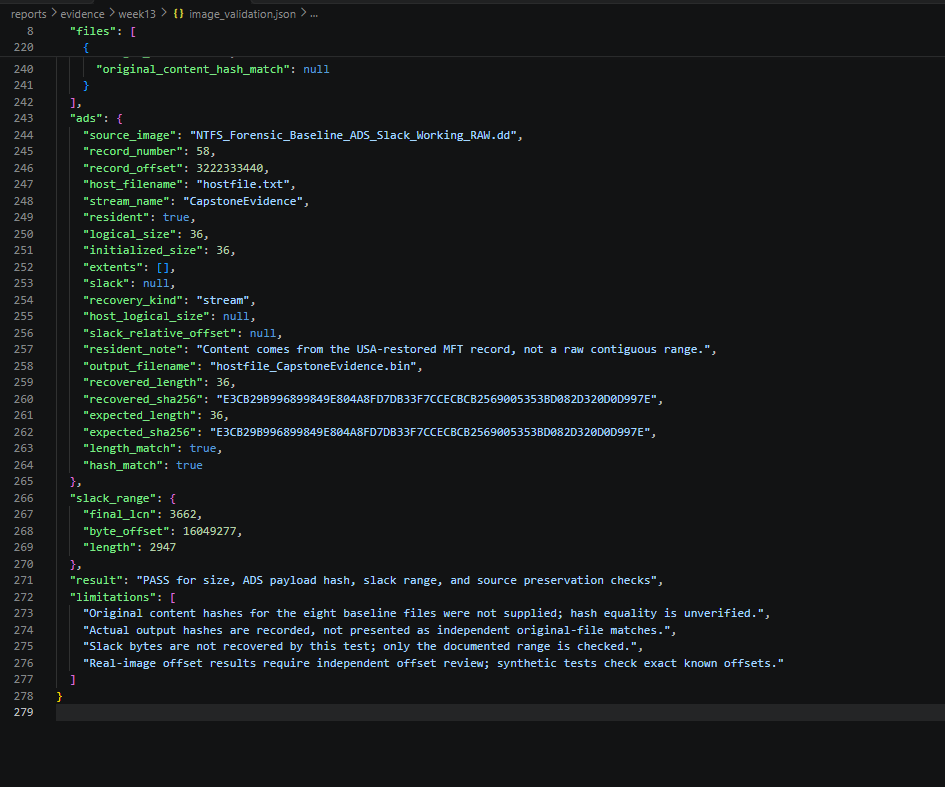
\includegraphics[width=\textwidth,height=6.8in,keepaspectratio]{w13_ads_validation.png}
\caption{Historical ADS validation evidence from November 15 showing the named stream and hash match.}
\label{fig:adsproof}\end{figure}

The document in record 41 had 13,437 logical bytes and 16,384 allocated bytes.
Its final content cluster left 2,947 slack bytes, beginning at absolute
offset 16,049,277, or hexadecimal \file{0x00F4E47D}. The requested 25-byte
marker was recovered with matching expected length and SHA-256.
Figure \ref{fig:slackproof} shows the bounded result, including the source
hash checks. The host document and slack payload are different exports.

\begin{figure}[p]\centering
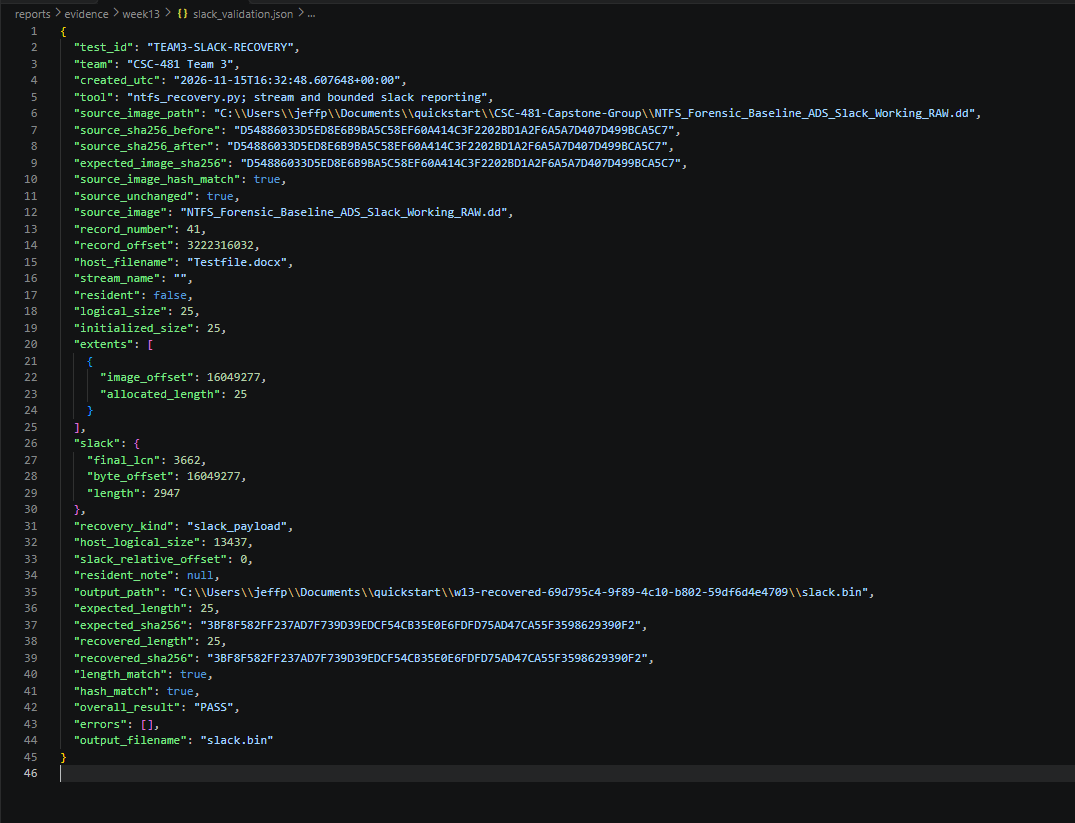
\includegraphics[width=\textwidth,height=6.8in,keepaspectratio]{w13_slack_validation.png}
\caption{Historical bounded-slack recovery evidence from November 15 with a 25-byte hash match.}
\label{fig:slackproof}\end{figure}

The working-image hash before and after the recorded recovery run was
identical. That observation supports preservation of the analyzed working
image during the run. It does not claim that the image equals the earlier
ADS-only source; the slack preparation intentionally changed its marker
range. The earlier full comparison records that preparation-stage difference.

\section{Capacity and Imperceptibility}
The measured Windows slack occupancy is 25/2,947 bytes, approximately
0.8483\%. Available capacity in that one tail is 2,947 bytes or 23,576 bits.
The ADS experiment demonstrates storage of 36 bytes or 288 bits; it does not
measure the maximum size of a named stream. These values describe filesystem
storage, so bits per pixel or audio sample would have no defined denominator.

No pixel or audio samples were modified, and no perceptual experiment was
performed. PSNR is therefore not applicable to the chosen carrier. The more
relevant preservation question is whether bytes outside the planned slack
range stayed the same and whether source images remained unchanged during
recovery. Historical full-copy comparison and image hashes provide evidence
for those questions. They do not constitute a human-perception or antivirus
evasion score.

\section{Synthetic Campaign and Robustness}
All 50 unchanged synthetic samples were recovered exactly and agreed with
the direct-byte-read baseline. All had zero bit errors. The five payload
sizes cover a one-byte minimum, the laboratory marker length, two intermediate
points, and the exact 324-byte synthetic tail boundary. Figure
\ref{fig:capacity} plots selected occupancy, while Table \ref{tab:campaign}
summarizes the paired clean and modified results.

\begin{table}[htbp]\centering
\caption{Synthetic campaign results with ten samples at each payload length.}
\label{tab:campaign}
\begin{tabular}{rrrrr}\toprule
Bytes & Occupancy \% & Exact clean & Changed hash failures & Changed BER \%\\\midrule
1 & 0.3086 & 10/10 & 10/10 & 12.5000\\
25 & 7.7160 & 10/10 & 10/10 & 0.5000\\
100 & 30.8642 & 10/10 & 10/10 & 0.1250\\
200 & 61.7284 & 10/10 & 10/10 & 0.0625\\
324 & 100.0000 & 10/10 & 10/10 & 0.0386\\\bottomrule
\end{tabular}\end{table}

\begin{figure}[htbp]\centering
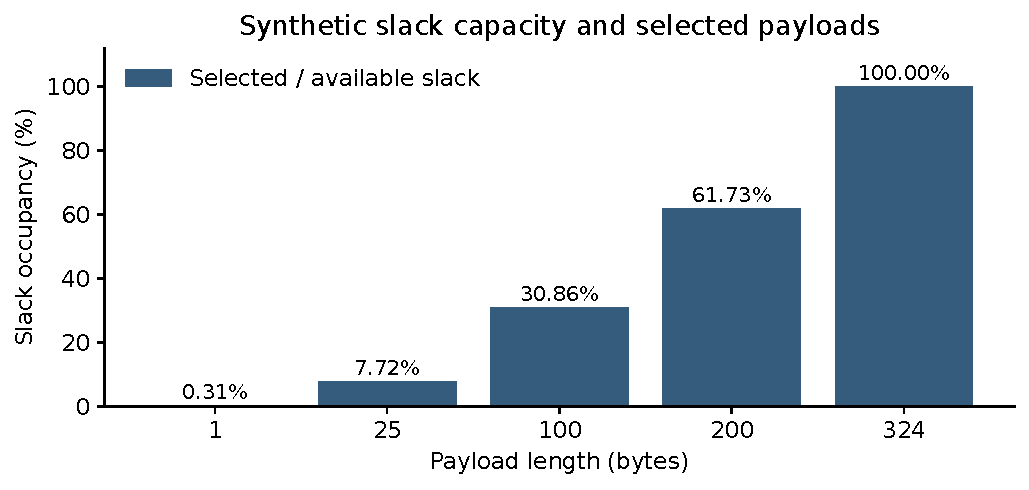
\includegraphics[width=0.94\textwidth]{capacity.pdf}
\caption{Payload occupancy in the 324-byte synthetic slack tail.}
\label{fig:capacity}\end{figure}

The deliberate one-bit changes were not corrected: the recovered bytes
contained exactly that one changed bit and the original-payload comparison
failed. Figure \ref{fig:ber} shows that the BER percentage falls as payload
length grows, even though every modified case contains the same number of
wrong bits. A small BER can therefore coexist with a decisive hash failure.
This is detection of corruption against a trusted expectation, not
steganographic recovery resilience after compression or file copying.

\begin{figure}[htbp]\centering
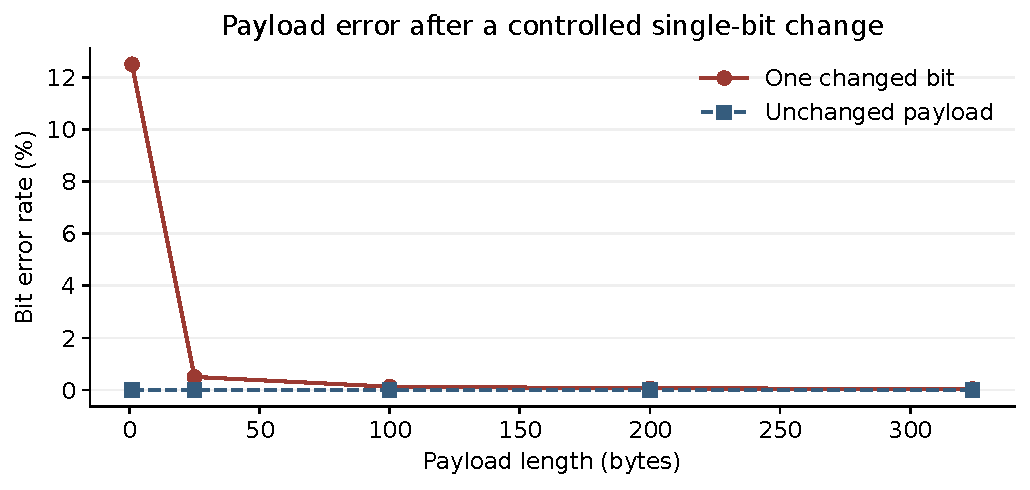
\includegraphics[width=0.94\textwidth]{ber.pdf}
\caption{Measured bit error rates after one deliberate stored-bit change.}
\label{fig:ber}\end{figure}

No corruption was introduced into the source used by each individual
recovery run. Modified images were created as separate inputs and given
their own correct expected image hash. This experimental control explains
why a modified case can have \file{source_unchanged=true} while its payload
hash fails: the source remained stable during recovery, but its payload no
longer matched the earlier original.

\section{Comparative Analysis}
The executed baseline seeks to the construction-known slack offset and
reads the specified length directly. It matched all 50 originals, as did
the structured recovery path. Their observed correctness difference on this
known-offset task is therefore zero percentage points. The structured tool's
additional behavior is metadata-based location, range validation, destination
protection, and saved verification; the baseline assumes location and length
are already correct.

That baseline is intentionally limited. It is not an independent NTFS parser
and does not validate the tool's behavior on unknown layouts. Nor is it a
performance comparison with The Sleuth Kit, Autopsy, Streams, or PhotoRec.
Timing columns are retained in the raw CSV, but single tiny cached reads
and a routine performing hashing, parsing, and report writes are not
equivalent workloads. We make no speed or scalability claim from them.

\section{Measured Detection and Evasion}
The separate November 25 detection experiment completed all 100 synthetic
cases. Table \ref{tab:detection} reports each fixed rule separately; the two
groups are not pooled into a general classifier score. Each group contains
25 intentionally hidden positives and 25 legitimate or ordinary negatives.

\begin{table}[htbp]\centering
\caption{Measured detection outcomes on constructed known-record inputs.}
\label{tab:detection}
\begin{tabular}{lrr}\toprule
Measure & ADS screening & Slack signature\\\midrule
True positives & 25 & 15\\
False negatives & 0 & 10\\
False positives & 10 & 0\\
True negatives & 15 & 25\\
Accuracy (\%) & 80 & 80\\
Detection rate (\%) & 100 & 60\\
False-positive rate (\%) & 40 & 0\\
Evasion rate (\%) & 0 & 40\\\bottomrule
\end{tabular}\end{table}

Named-stream screening detected all 25 deliberately hidden ADS cases.
It also flagged all ten legitimate named-stream controls; the 15 ordinary
files were not flagged. Thus stream presence is a useful review signal but
does not establish concealment intent. Its 40\% false-positive rate refers
to the hidden-content label, not an error locating the legitimate streams.

The slack rule detected all 15 plaintext markers, including placements at
varied offsets in the calculated tail. It missed all ten XOR-transformed
markers. All 25 negatives were correctly rejected, including ten with the
literal marker in logical file content rather than slack. The resulting
40\% evasion rate shows the fixed signature's dependence on unchanged bytes;
it does not show resistance to broader forensic inspection or other signatures.

\begin{figure}[htbp]\centering
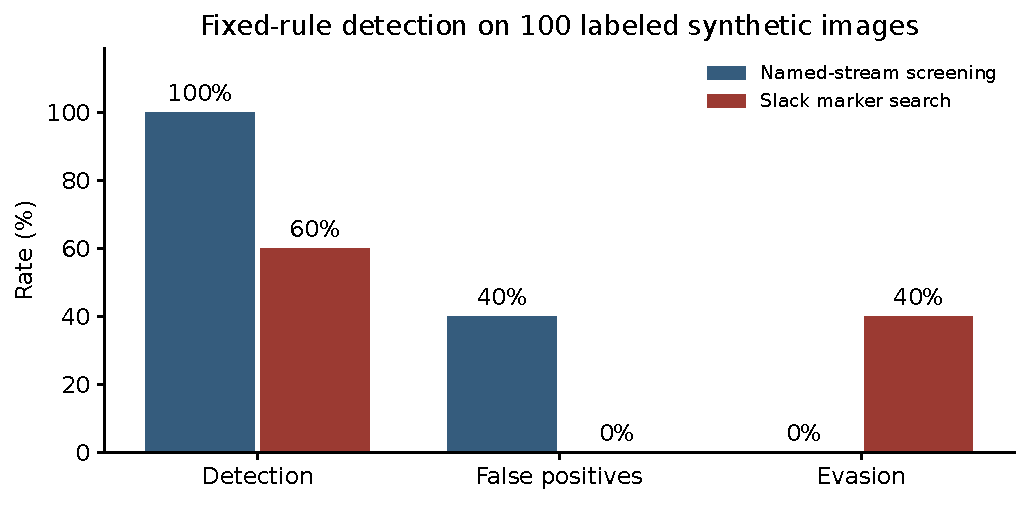
\includegraphics[width=0.94\textwidth]{detection.pdf}
\caption{Detection and evasion rates measured separately for two fixed rules.
Each rule was tested on 50 synthetic images.}
\label{fig:detection}\end{figure}

Both rules also flagged their known positives in the original Windows
working image: record 58 contained \file{CapstoneEvidence}, and record 41's
calculated slack contained the marker at relative offset zero. The image's
full SHA-256 matched the recorded expectation before and after screening.
All 100 synthetic image hashes were also unchanged. These two Windows
positives do not provide a real-volume false-positive estimate.

The fixed scenario proportions, shared metadata layout, known target records,
and known slack signature limit external validity. No rule was fitted or tuned
using the outcomes. The measured percentages describe this challenge set;
they are not estimates of hidden-content prevalence or detection accuracy
across arbitrary Windows volumes. Raw labels, decisions, hashes, and summary
are retained under \file{reports/evidence/final_detection/}.

\section{Regression Results and Evidence Limits}
The November 15 suite passed 64 tests in 4.729 seconds. The November 24
clean-copy release check passed 68 tests in 8.613 seconds, plus seven
acceptance checks. The four added tests cover deterministic data generation,
refusal of an existing dataset directory, end-to-end verification, and CLI
execution from an unrelated directory. Runtime differences cannot be
attributed to a performance regression because workload and execution
conditions differ.

The November 25 report extension passed all 73 tests in 9.567 seconds,
including five additional detection-campaign tests. This extends the current
report branch; it does not change the earlier tagged release's test count.

The strongest measured results are the two historical original-marker hash
matches and exact recovery in the constructed campaign. The team additionally
confirmed all eight baseline-file hash matches on November 25. Broad real-volume
coverage and realistic attack survival remain limited. The new labeled
detection experiment supplies rule-specific accuracy, false-positive, and
evasion measurements. General discovery of unknown hidden material remains
unvalidated. The results support controlled recovery and a bounded screening
comparison, rather than universal forensic discovery or covert security.

\chapter{Security and Robustness Analysis}
\section{Attack Surface Analysis}
\subsection{Payload Removal or Overwrite}
An actor with permission to alter the storage can remove a named stream,
replace its contents, or overwrite the bytes holding the slack marker. A
slack marker also depends on allocation remaining compatible with the
recorded location. The current implementation does not reserve the slack
through an active filesystem service and does not provide an error-correcting
code. Once the selected original bytes are lost, knowing their earlier hash
does not reconstruct them.

The single-bit experiments demonstrate a narrow consequence: recovery still
exports the requested length, but original-payload verification fails. They
do not establish a measured survival rate after mounted filesystem writes,
defragmentation, backup, copying to another filesystem, or secure deletion.
Those transformations would require new controlled images and independent
recording of their effects. For current evidence, stable offline storage is
an assumption, not a robustness feature.

\subsection{Manifest Substitution and Misleading Expectations}
The original hash is a trust anchor. If an attacker replaces both a payload
and the manifest used to judge it, matching those two values does not
establish agreement with the earlier legitimate content. SHA-256 digests
identify changes relative to a reference \cite{sha}; they are not signatures
proving the reference's author. The project's plaintext JSON manifests are
not cryptographically authenticated.

This attack is feasible wherever a person can edit both the evidence copy
and its expectations. Repository history offers a review trail, but an
investigator still needs to establish which version is trusted. A useful
hardening step would be to sign acquisition manifests and store the original
digest record separately. That would address provenance and substitution;
it would not hide the marker or improve NTFS parsing coverage.

\subsection{Malformed Metadata and Resource Exhaustion}
A hostile image can supply inconsistent lengths, invalid mapping pairs,
out-of-volume extents, unsupported flags, or damaged update sequences. These
structures can lead to false content, excessive work, or unexpected reads if
interpreted without checks. The recovery layer validates many such cases and
the suite includes malformed and truncated inputs. Unsupported layouts are
refused instead of treated as successful empty files.

The implementation has not undergone comprehensive fuzzing, formal
verification, or independent adversarial review. Some valid-looking metadata
can still request substantial work, and a full-image hash costs a read of
the entire input. Controlled fixtures do not establish resistance to every
resource-exhaustion attack. Operational hardening would include explicit
resource budgets, controlled process execution, and a documented policy for
very large images.

\subsection{Source Changes During Examination}
Before/after hashing is an observation over two points in time. It does not
hold a transactionally immutable snapshot throughout the export. If another
process changes the source while the tool is running, reads can observe an
inconsistent state. The code warns against changing the image between
location and recovery; the report can mark a changed-source hash as failure.
An adversary able to change and restore a file between checks is outside the
protection offered by those two hashes alone.

The appropriate mitigation is acquisition and stable-image handling, with
read-only media or a protected snapshot where available. A reproducible
student experiment should not be described as a hardware write-blocking
system or a complete chain-of-custody solution. NIST's forensic guidance
provides the wider process context for preserving and interpreting evidence
\cite{nist86}.

\section{Detection and Confidentiality Limits}
The markers are plain ASCII and the stream name is documented. The design
does not attempt to defeat an examiner who enumerates named streams or reads
the relevant slack bytes. The reviewed Streams and Sleuth Kit capabilities
illustrate why omission from a default file view is not equivalent to
undetectability \cite{sysstreams,icat}. Our results should therefore be read
as evidence that such material can be recovered, not that the hiding method
evades capable forensic tools.

No encryption protects the hidden content. Microsoft's EFS is a distinct
filesystem encryption feature \cite{efs}, and it is outside this extractor's
supported stream types. Adding application-level encryption in a future
experiment would address confidentiality of the payload, but would not make
its existence inherently invisible. Verification of plaintext recovery would
then require a clearly specified decryption stage and key-handling procedure.

\section{Implementation and Evaluation Limitations}
The release's recovery path applies fixups before interpreting resident
content. The older metadata CLI does not apply those checks on every path;
its output must not be treated as equivalent to a validated content export.
Fragmented ordinary streams are tested, whereas general fragmented MFT
traversal is refused. Extension records, attribute lists, sparse/compressed/
encrypted recovery, GPT, complete directory reconstruction, and unknown
payload discovery are not demonstrated.

The team confirmed baseline-file hash matches on November 25.
The 50 new samples share one handcrafted metadata layout.
Recovery-corruption testing was limited to a single-bit substitution.
The separate 100-image detection campaign measured fixed-rule false-positive
and evasion rates, including misses for a reversible marker transformation.
It did not measure unknown-content discovery across independent real volumes.
No benchmark established general extraction throughput. These limits prevent
broad security or compatibility claims even though all included tests passed.

\section{Future Hardening}
The first priority is a broader independent validation corpus: multiple
Windows-formatted images, varied cluster sizes and fragmentation, and
original hashes collected before extraction. A second priority is shared
strict record validation across both CLIs, followed by bounded MFT-run and
attribute-list support. Those changes should be tested against independent
tools and retained failure cases.

Signed manifests would strengthen provenance. Mutation testing and fuzzing
would exercise parser defenses. Separate real-filesystem copy-and-write
tests should measure payload loss. Encryption alone would not resolve these
evidence and parsing limitations.

\chapter{Conclusion and Future Work}
\section{Conclusion}
The project achieved its main controlled-recovery aim. A Python raw-image
workflow identifies the relevant NTFS structures, selects documented named
streams and final-cluster slack ranges, exports recovered bytes to separate
files, and records verification outcomes. The two original hidden markers
were recovered with matching expected lengths and SHA-256 values, while the
recorded working-image hash remained unchanged during recovery.

Objective 1 was achieved for the documented unencrypted laboratory image:
partition geometry and MFT location were recorded and compared with Windows
output. Objective 2 was achieved for all eight baseline-file names and lengths.
The team also confirmed matching original and recovered SHA-256 hashes
for all eight files on November 25. This later confirmation is recorded
separately from the earlier machine-generated recovery results.

Objectives 3 and 4 were achieved for the documented ADS and slack payloads.
Their original expectations and selection identities were preserved, and
later exports matched them. Objective 5 is supported by 68 passing release
tests, seven acceptance checks, and the final synthetic campaign. The
campaign recovered 50 unchanged payloads exactly and detected 50 deliberate
single-bit mismatches against the original expectations. These outcomes
demonstrate correctness on tested inputs, not immunity to every attack.

A separate 100-image detection campaign measured 100\% ADS detection with
40\% false positives and 0\% evasion, versus 60\% slack-marker detection with
0\% false positives and 40\% evasion. These fixed-rule results expose the
tradeoff between broad stream screening and a narrow plaintext signature.

Objective 6 was achieved through the tagged source package, updated README,
and small generated dataset. A fresh source copy ran without the separately
retained 8 GB images. The final report adds its own reproducible campaign
and raw results while preserving the identity of the earlier code release.
The project can therefore be considered successful within its stated
educational scope, with partial rather than universal validation.

Filename, length, original-payload hash, and source-preservation checks
support different conclusions. Each is reported separately.

\section{Future Work}
Three extensions would provide the most practical improvement:
\begin{enumerate}
\item Build a diverse Windows-created corpus with original hashes, several
allocation patterns, and independent recovery comparisons. This would
address the current concentration on one lab volume and one synthetic layout.
\item Extend strict validation consistently to the metadata CLI and implement
bounded fragmented-MFT and attribute-list handling. Each newly supported
layout should have a positive case, malformed cases, and explicit limits.
\item Extend robustness and discovery studies to independent Windows-created
positive and negative volumes. Evaluate copying, filesystem writes, and payload
removal separately from signature evasion, and compare broader detectors with
the two measured screening baselines using defined denominators.
\end{enumerate}

These extensions preserve the existing emphasis on transparent evidence.
They would broaden the tool's usefulness without requiring unsupported
claims about covert security or operational forensic readiness.

\section{Self Evaluation}
\noindent\textbf{Jeff Perez self-assigned grade: B (85/100).}

This assessment credits implementation of the parser, recovery support,
controlled slack-copy tool, verification reporting, automated tests, and
reproducible release package. Documented results demonstrate recovery of
both hidden markers and protection of the source image. Deductions reflect
limited independent real-volume validation, unsupported advanced NTFS
layouts, and the need for broader robustness and discovery experiments.
Completing the planned functionality is a substantial result, while the
remaining evaluation gaps justify a B rather than full marks.

\newpage
\noindent\textbf{Lucas Curtis self-assigned grade: A (95/100).}

This assessment credits preparation of the VirtualBox laboratory, image
exports, known-file information, the manual ADS procedure, recovery-workflow
documentation, evidence organization, and the initial final-report and
evidence-log drafts. These contributions supplied the controlled environment
and records needed to connect implementation with observed results.
Deductions acknowledge limited test-volume diversity and incomplete
historical environment details. The contribution record in Appendix C
provides the supporting development history.

\clearpage
\begin{thebibliography}{20}
\addcontentsline{toc}{chapter}{References}
\bibitem{streams} Microsoft, ``File streams (local file systems).''
\url{https://learn.microsoft.com/en-us/windows/win32/fileio/file-streams}.
\bibitem{clusters} Microsoft, ``Files and clusters.''
\url{https://learn.microsoft.com/en-us/windows/win32/fileio/files-and-clusters}.
\bibitem{anderson} R. Anderson, ``Stretching the limits of steganography,'' in
\emph{Information Hiding}, LNCS 1174, 1996, pp. 39--48. Author manuscript.
\url{https://www.cl.cam.ac.uk/archive/rja14/Papers/stegan.pdf}.
\bibitem{nist86} K. Kent, S. Chevalier, T. Grance, and H. Dang,
\emph{Guide to Integrating Forensic Techniques into Incident Response},
NIST SP 800-86, Aug. 2006. \url{https://doi.org/10.6028/NIST.SP.800-86}.
\bibitem{petitcolas} F. A. P. Petitcolas, ``The information hiding homepage.''
\url{https://www.petitcolas.net/steganography/}.
\bibitem{mft} Microsoft, ``Master File Table,'' Windows developer notes.
\url{https://learn.microsoft.com/en-us/windows/win32/devnotes/master-file-table}.
\bibitem{record} Microsoft, ``FILE\_RECORD\_SEGMENT\_HEADER structure.''
\url{https://learn.microsoft.com/en-us/windows/win32/devnotes/file-record-segment-header}.
\bibitem{attribute} Microsoft, ``ATTRIBUTE\_RECORD\_HEADER structure.''
\url{https://learn.microsoft.com/en-us/windows/win32/devnotes/attribute-record-header}.
\bibitem{usa} Microsoft, ``MULTI\_SECTOR\_HEADER structure.''
\url{https://learn.microsoft.com/en-us/windows/win32/devnotes/multi-sector-header}.
\bibitem{standard} Microsoft, ``STANDARD\_INFORMATION structure.''
\url{https://learn.microsoft.com/en-us/windows/win32/devnotes/standard-information}.
\bibitem{filename} Microsoft, ``FILE\_NAME structure.''
\url{https://learn.microsoft.com/en-us/windows/win32/devnotes/file-name}.
\bibitem{fsutilfile} Microsoft, ``Fsutil file.''
\url{https://learn.microsoft.com/en-us/windows-server/administration/windows-commands/fsutil-file}.
\bibitem{sysstreams} M. Russinovich, ``Streams,'' Microsoft Sysinternals.
\url{https://learn.microsoft.com/en-us/sysinternals/downloads/streams}.
\bibitem{tsk} The Sleuth Kit, ``File and volume system analysis.''
\url{https://www.sleuthkit.org/sleuthkit/desc.php}.
\bibitem{icat} The Sleuth Kit, ``ICAT(1) manual page.''
\url{https://sleuthkit.org/sleuthkit/man/icat.html}.
\bibitem{photorec} CGSecurity, ``PhotoRec.''
\url{https://www.cgsecurity.org/wiki/PhotoRec}.
\bibitem{cftt} National Institute of Standards and Technology,
``Computer Forensics Tool Testing Program.''
\url{https://www.nist.gov/itl/csd/secure-systems-and-applications/computer-forensics-tool-testing-program-cftt}.
\bibitem{sha} National Institute of Standards and Technology,
\emph{Secure Hash Standard}, FIPS 180-4, Aug. 2015.
\url{https://doi.org/10.6028/NIST.FIPS.180-4}.
\bibitem{fsinfo} Microsoft, ``Fsutil fsinfo.''
\url{https://learn.microsoft.com/en-us/windows-server/administration/windows-commands/fsutil-fsinfo}.
\bibitem{efs} Microsoft, ``File encryption.''
\url{https://learn.microsoft.com/en-us/windows/win32/fileio/file-encryption}.
\end{thebibliography}
\noindent Online documentation accessed November 24, 2026.

\appendix
\chapter{User Manual and Quick Start Guide}
\section{Installation and Release Selection}
Install Git and Python 3.11 or later. These Windows commands use \file{py};
use your Python executable elsewhere. No third-party runtime packages are needed.
\begin{lstlisting}
git clone https://github.com/Lcurtis1Broncos/CSC-481-Capstone-Group.git
cd CSC-481-Capstone-Group
git checkout v1.0-final
py -m unittest discover -s tests -v
py tests/verify_submission.py submission_check
\end{lstlisting}
The acceptance script generates inputs, invokes the CLIs, and saves outputs
and reports. All seven checks should pass. Always choose a new output folder.

\section{Inspecting the Generated Image}
To create only the portable dataset and inspect its records:
\begin{lstlisting}
py tests/generate_submission_dataset.py generated_dataset
py code/ntfs_image_reader.py generated_dataset/synthetic.dd --list-files 8 --show-record 1 --show-record 2
py code/ntfs_recovery.py generated_dataset/synthetic.dd --record 2 --stream CapstoneEvidence --output new_ads.bin
\end{lstlisting}
The final command exports and hashes the ADS. The acceptance script adds
original expectations and a saved report to establish a verified PASS.

\section{Reproducing the Report Campaign}
From the report branch, which adds the campaign after the code tag, run:
\begin{lstlisting}
py tests/run_report_campaign.py report_campaign_new
\end{lstlisting}
Expected results are 50 exact recoveries, 50 baseline matches, and 50
single-bit hash failures. Originals, paired inputs, reports, and CSV results
are saved in the new folder.

For the separate detection experiment on the report branch:
\begin{lstlisting}
py tests/run_detection_campaign.py detection_campaign_new
\end{lstlisting}
This creates 100 labeled inputs, a manifest, \file{results.csv}, and
\file{summary.json}. To repeat the two Windows positive checks as well,
add \file{--lab-image} followed by the preserved working-image path.
This optional step hashes the entire large image twice. Recorded results,
the 73-test log, a result figure, and reproduction details are retained under
\file{reports/evidence/final_detection/}. The earlier code tag does not
contain either report campaign.

\section{Historical Windows Image Commands}
These commands require the separately retained Windows image. Set the
PowerShell variable to its actual path first.
\begin{lstlisting}
$IMAGE = "path/to/NTFS_Forensic_Baseline_ADS_Slack_Working_RAW.dd"
py code/ntfs_image_reader.py $IMAGE --show-record 41 --show-record 58
py code/ntfs_recovery.py $IMAGE --record 58 --stream CapstoneEvidence --output new_lab_ads.bin
py code/ntfs_recovery.py $IMAGE --record 41 --slack-length 25 --output new_lab_slack.bin
\end{lstlisting}
For a saved verification decision, add these options with the original values:
\begin{lstlisting}
--report NEW_REPORT.json
--expected-length ORIGINAL_BYTE_COUNT
--expected-sha256 ORIGINAL_PAYLOAD_HASH
--expected-image-sha256 ORIGINAL_IMAGE_HASH
\end{lstlisting}
Appendix B records the hashes. Output parents must exist; destinations must
be new. Full-image hashing takes longer than locating content.

\section{Interpreting Decisions}
PASS requires the expected payload length and original hash to match, with
observed source preservation. FAIL indicates a mismatched expectation or
changed source. NOT\_VERIFIED means an original expectation was omitted.
Input or recovery errors are distinct from a failed content comparison.
The reporting CLI returns 0 for PASS, 1 for FAIL or NOT\_VERIFIED, and 2 for
input/recovery errors. Diagnostic or partial files after an error must not
be treated as completed evidence.

\chapter{Complete Raw Test Results}
\section{Marker and Image Hash Register}
\noindent\textbf{Working-image SHA-256:}\\
\workinghash

\medskip\noindent\textbf{ADS marker, 36 bytes:}\\
\file{CAPSTONE_ADS_TEST_20261001_Team3_001}\\
\texttt{E3CB29B996899849E804A8FD7DB33F7CC}\\
\texttt{ECBCB2569005353BD082D320D0D997E}

\medskip\noindent\textbf{Slack marker, 25 bytes:}\\
\file{TEAM3_SLACK_TEST_20261008}\\
\texttt{3BF8F582FF237AD7F739D39EDCF54CB35E}\\
\texttt{0E6FDFD75AD47CA55F3598629390F2}

\medskip\noindent Windows slack location: record 41, absolute byte offset
16,049,277; available tail 2,947 bytes; selected payload 25 bytes.
These markers and their hashes precede the later recovery comparisons.
The portable fixture uses the same marker strings but a different image
and geometry; its image hash must not be confused with the Windows image.

\section{Baseline File Hash Register}
The November 15 recovery recorded the hashes below. On November 25, Jeff confirmed that the original-file hashes match all eight recorded values. Original values are reproduced on that team confirmation; original command output was not attached. The dated confirmation is stored in reports/evidence/final\_report/baseline\_hash\_confirmation.json.
\begin{longtable}{p{1.6in}p{4.4in}}
\caption{Original and recovered SHA-256 values confirmed equal for all eight files.}\\
\toprule File & Original and recovered SHA-256\\\midrule\endfirsthead
\toprule File & Original and recovered SHA-256\\\midrule\endhead
Test.txt & \texttt{D68EC557336622896727E44ED0031366}\newline\texttt{62FCD67CE8F9F57B23E70C0E09ADA797}\\[0.6em]
Test2.txt & \texttt{BA7F25F70009A6D45A9EF88C857C9C35}\newline\texttt{7856AA6D1201486DE9070522CFAEE64E}\\[0.6em]
Testfile.docx & \texttt{84A8A7AC155C36A5F4F9196A412D8DB1}\newline\texttt{6A6F12BD10794FEC362542E562DBE347}\\[0.6em]
SunflowerTest.jpg & \texttt{658C1F66CE1C2D05B51F4E2004498122}\newline\texttt{8AAE39BE33B14737B5ADD448378B9E7C}\\[0.6em]
Thetestfile.pdf & \texttt{61FCC2B322094257A6B845E15D7AEFF9}\newline\texttt{9564E83260EA413DB05180DD8A0E3C8C}\\[0.6em]
WaterfallTest.png & \texttt{19CE26BC665962B8B6B766C48EFFC867}\newline\texttt{6D1191B7B46CACD165418892ED42AA08}\\[0.6em]
HTMLtestdoc.html & \texttt{815246781F0ADE404A0FECD2531CB027}\newline\texttt{AB7F6C1177868967BC7CCA47D88AE0FB}\\[0.6em]
JSON\_test\_File.json & \texttt{65EAF0824C357D4FC9955E75CA29CF3F}\newline\texttt{6476DCB0374241DAB08C3714991E8D34}\\[0.6em]
\bottomrule\end{longtable}
\section{All Synthetic Payload Samples}
Each row represents a separately generated payload. Clean recovery and the direct-read baseline matched exactly in every row. Each changed case contains one deliberately flipped bit and a failed original-payload hash comparison.
\begin{longtable}{rrrrrr}
\caption{Complete 50-sample synthetic campaign results.}\\
\toprule ID & Bytes & Clean BER \% & Changed BER \% & Exact baseline & Hash failure\\\midrule\endfirsthead
\toprule ID & Bytes & Clean BER \% & Changed BER \% & Exact baseline & Hash failure\\\midrule\endhead
1 & 1 & 0 & 12.500000 & Yes & Yes\\
2 & 25 & 0 & 0.500000 & Yes & Yes\\
3 & 100 & 0 & 0.125000 & Yes & Yes\\
4 & 200 & 0 & 0.062500 & Yes & Yes\\
5 & 324 & 0 & 0.038580 & Yes & Yes\\
6 & 1 & 0 & 12.500000 & Yes & Yes\\
7 & 25 & 0 & 0.500000 & Yes & Yes\\
8 & 100 & 0 & 0.125000 & Yes & Yes\\
9 & 200 & 0 & 0.062500 & Yes & Yes\\
10 & 324 & 0 & 0.038580 & Yes & Yes\\
11 & 1 & 0 & 12.500000 & Yes & Yes\\
12 & 25 & 0 & 0.500000 & Yes & Yes\\
13 & 100 & 0 & 0.125000 & Yes & Yes\\
14 & 200 & 0 & 0.062500 & Yes & Yes\\
15 & 324 & 0 & 0.038580 & Yes & Yes\\
16 & 1 & 0 & 12.500000 & Yes & Yes\\
17 & 25 & 0 & 0.500000 & Yes & Yes\\
18 & 100 & 0 & 0.125000 & Yes & Yes\\
19 & 200 & 0 & 0.062500 & Yes & Yes\\
20 & 324 & 0 & 0.038580 & Yes & Yes\\
21 & 1 & 0 & 12.500000 & Yes & Yes\\
22 & 25 & 0 & 0.500000 & Yes & Yes\\
23 & 100 & 0 & 0.125000 & Yes & Yes\\
24 & 200 & 0 & 0.062500 & Yes & Yes\\
25 & 324 & 0 & 0.038580 & Yes & Yes\\
26 & 1 & 0 & 12.500000 & Yes & Yes\\
27 & 25 & 0 & 0.500000 & Yes & Yes\\
28 & 100 & 0 & 0.125000 & Yes & Yes\\
29 & 200 & 0 & 0.062500 & Yes & Yes\\
30 & 324 & 0 & 0.038580 & Yes & Yes\\
31 & 1 & 0 & 12.500000 & Yes & Yes\\
32 & 25 & 0 & 0.500000 & Yes & Yes\\
33 & 100 & 0 & 0.125000 & Yes & Yes\\
34 & 200 & 0 & 0.062500 & Yes & Yes\\
35 & 324 & 0 & 0.038580 & Yes & Yes\\
36 & 1 & 0 & 12.500000 & Yes & Yes\\
37 & 25 & 0 & 0.500000 & Yes & Yes\\
38 & 100 & 0 & 0.125000 & Yes & Yes\\
39 & 200 & 0 & 0.062500 & Yes & Yes\\
40 & 324 & 0 & 0.038580 & Yes & Yes\\
41 & 1 & 0 & 12.500000 & Yes & Yes\\
42 & 25 & 0 & 0.500000 & Yes & Yes\\
43 & 100 & 0 & 0.125000 & Yes & Yes\\
44 & 200 & 0 & 0.062500 & Yes & Yes\\
45 & 324 & 0 & 0.038580 & Yes & Yes\\
46 & 1 & 0 & 12.500000 & Yes & Yes\\
47 & 25 & 0 & 0.500000 & Yes & Yes\\
48 & 100 & 0 & 0.125000 & Yes & Yes\\
49 & 200 & 0 & 0.062500 & Yes & Yes\\
50 & 324 & 0 & 0.038580 & Yes & Yes\\
\bottomrule\end{longtable}
\section{Release Regression Output}
The following complete output is the November 24 clean-copy release test run. The seven acceptance checks are recorded in the accompanying verification JSON.
\lstinputlisting[basicstyle=\ttfamily\scriptsize]{../evidence/final_code/regression.txt}
\section{Acceptance Summary}
\lstinputlisting[basicstyle=\ttfamily\scriptsize]{../evidence/final_code/verification.json}


\section{Detection Campaign: All 100 Decisions}
The following raw CSV retains every construction label, prediction, outcome,
and source-preservation decision from November 25. The header identifies the
columns. True means a present hidden payload, a flag, or unchanged source as
appropriate. Interpret the two screening groups separately using Chapter 5's
denominators; this file is not a recovery-hash comparison.
\lstinputlisting[basicstyle=\ttfamily\scriptsize]{../evidence/final_detection/results.csv}

\section{Raw Artifact Locations}
The repository retains the full historical image and slack validation JSON
under \file{reports/evidence/week13/}, release output under
\file{reports/evidence/final_code/}, and all 50 campaign rows with timing
columns under \file{reports/evidence/final_report/results.csv}.
The campaign generator recreates individual originals, images, outputs,
and reports; those generated binaries need not be stored in Git. The
historical evidence catalog contains additional image-state hashes,
screenshots, and hexdumps.

\chapter{Development Log and Contribution Record}
\section{Version History Summary}
The table below was generated from non-merge commits reachable from the
report branch's starting point, through November 24. Merge commits are
excluded to avoid counting integration as another implementation change.
Jeff's historical identities are grouped together; the Lucas identity is
\file{Lcurtis1Broncos}. Counts are evidence of recorded activity, not
measurements of effort, quality, or a prescribed individual grade.
The underlying dated commit list is retained in
\file{reports/evidence/final_report/commit_history.txt}.

\begin{longtable}{lrrr}
\caption{Non-merge commits by week and recorded author identity.}\\
\toprule Week beginning & Jeff identities & Lucas identity & Other\\\midrule\endfirsthead
\toprule Week beginning & Jeff identities & Lucas identity & Other\\\midrule\endhead
2026-08-17 & 3 & 6 & 0\\
2026-08-24 & 1 & 2 & 0\\
2026-08-31 & 13 & 19 & 0\\
2026-09-07 & 5 & 7 & 0\\
2026-09-14 & 4 & 4 & 0\\
2026-09-21 & 2 & 1 & 0\\
2026-09-28 & 1 & 6 & 0\\
2026-10-05 & 1 & 0 & 0\\
2026-10-12 & 1 & 0 & 0\\
2026-10-19 & 1 & 1 & 0\\
2026-10-26 & 2 & 5 & 0\\
2026-11-02 & 1 & 5 & 0\\
2026-11-09 & 2 & 16 & 0\\
2026-11-16 & 0 & 4 & 0\\
2026-11-23 & 1 & 0 & 0\\
\bottomrule\end{longtable}


\section{Contribution Summary}
Lucas prepared the dedicated VirtualBox laboratory, supplied image exports
and known-file information, documented the manual ADS procedure, and added
ADS/slack workflow records, an evidence catalog, and the initial final-report
and evidence-log drafts. His repository activity also records review,
documentation updates, and integration of weekly work.

Jeff implemented the boot and MFT parser, attribute and run interpretation,
controlled slack-copy tool, recovery support and verification reporting,
automated tests, and release packaging. He recorded parser and payload
validation evidence and assembled weekly documentation. Jeff also prepared
the November 24 report campaign and expanded report.

The meeting records and journals provide context alongside commits. The
semester plan's midterm interval was adjusted after the actual deadline
required submission on October 11. The following week was used for validation
and planning. Later work progressed through recovery, ADS checks, slack
checks, consolidated testing, and final evidence/report preparation. This
sequence is visible in the dated source history and weekly evidence.

\section{Repository Contents}
The tagged code package includes source modules, tests and dataset generators,
README instructions, design notes, evidence, and weekly documentation. The
report branch adds the final report source, figures, campaign generator, and
raw campaign tables. Large original images and personal lesson exports
remain outside Git. For the code assignment the immutable submission
reference is \file{v1.0-final}; the signed final report is a separate artifact.

\end{document}
